\documentclass[journal]{IEEEtran}
\usepackage{amsmath,amsthm}
\usepackage{iftex}
\ifXeTeX
  \usepackage{newtxmath}
  \usepackage[no-math]{fontspec}
  \setmainfont{texgyretermes}[Extension=.otf, UprightFont=*-regular, BoldFont=*-bold,
                              ItalicFont=*-italic, BoldItalicFont=*-bolditalic]
\else
  \usepackage[T1]{fontenc}
  \usepackage{newtxtext,newtxmath}
\fi
\usepackage{cite}
\usepackage{graphicx}
\usepackage{booktabs}
\usepackage{array}
\usepackage{xcolor}
\usepackage{tikz}
\usetikzlibrary{arrows.meta,positioning,calc}
\usepackage{url}
\usepackage{algorithm}
\usepackage{algpseudocode}
\usepackage{flafter}
\usepackage[hidelinks]{hyperref}

\algnewcommand{\IfThen}[2]{\State \algorithmicif\ #1\ \algorithmicthen\ #2}
\definecolor{fgblue}{HTML}{2A78D6}
\definecolor{fgorange}{HTML}{EB6834}
\definecolor{fgink}{HTML}{0B0B0B}
\definecolor{fgmuted}{HTML}{898781}
\definecolor{fgfill}{HTML}{EEF4FC}
\definecolor{fggrey}{HTML}{F4F3F0}

% supplementary numbering: Section S1, Fig. S1, Table S1, Algorithm S1
\renewcommand{\thesection}{S\arabic{section}}
\renewcommand{\thefigure}{S\arabic{figure}}
\renewcommand{\thetable}{S\arabic{table}}
\renewcommand{\thealgorithm}{S\arabic{algorithm}}

% Generated by experiments/make_figures.py - do not edit by hand.
\newcommand{\lfwImages}{13,233}
\newcommand{\lfwPeople}{5,749}
\newcommand{\lfwPeopleTen}{158}
\newcommand{\lfwPeopleTwenty}{62}
\newcommand{\lfwMultiFace}{2,777}
\newcommand{\lfwFaceWidth}{93}
\newcommand{\lfwYawMedian}{7.2}
\newcommand{\lfwYawNinety}{18.4}
\newcommand{\lfwAccFull}{99.43}
\newcommand{\lfwStdFull}{0.33}
\newcommand{\lfwAucFull}{0.9988}
\newcommand{\lfwEerFull}{0.73}
\newcommand{\lfwTarTwoFull}{99.40}
\newcommand{\lfwTarThreeFull}{98.93}
\newcommand{\lfwThrFull}{0.330}
\newcommand{\lfwGenFull}{0.664}
\newcommand{\lfwImpFull}{0.085}
\newcommand{\lfwAccNoTTA}{99.35}
\newcommand{\lfwStdNoTTA}{0.37}
\newcommand{\lfwAucNoTTA}{0.9988}
\newcommand{\lfwEerNoTTA}{0.80}
\newcommand{\lfwTarTwoNoTTA}{99.27}
\newcommand{\lfwTarThreeNoTTA}{98.80}
\newcommand{\lfwThrNoTTA}{0.313}
\newcommand{\lfwGenNoTTA}{0.654}
\newcommand{\lfwImpNoTTA}{0.084}
\newcommand{\lfwAccNoAlign}{87.88}
\newcommand{\lfwStdNoAlign}{1.13}
\newcommand{\lfwAucNoAlign}{0.9486}
\newcommand{\lfwEerNoAlign}{12.03}
\newcommand{\lfwTarTwoNoAlign}{62.93}
\newcommand{\lfwTarThreeNoAlign}{45.37}
\newcommand{\lfwThrNoAlign}{0.297}
\newcommand{\lfwGenNoAlign}{0.479}
\newcommand{\lfwImpNoAlign}{0.152}
\newcommand{\opGenuine}{52,904}
\newcommand{\opImpostor}{1,000,000}
\newcommand{\opImpMax}{0.555}
\newcommand{\opImpQ}{0.430}
\newcommand{\farRelaxed}{0.0628}
\newcommand{\frrRelaxed}{0.88}
\newcommand{\farBalanced}{0.0054}
\newcommand{\frrBalanced}{2.54}
\newcommand{\farStrict}{0.0004}
\newcommand{\frrStrict}{7.79}
\newcommand{\unkGenuine}{0.31}
\newcommand{\unkImpostor}{99.08}
\newcommand{\adaptiveFar}{0.0000}
\newcommand{\idPeople}{158}
\newcommand{\idImages}{4,324}
\newcommand{\idOneNn}{99.30}
\newcommand{\idTwoNn}{99.84}
\newcommand{\idTwoTopthree}{99.89}
\newcommand{\idTwoTopfive}{99.89}
\newcommand{\idTwoCentroid}{99.89}
\newcommand{\idThreeNn}{99.88}
\newcommand{\idThreeTopthree}{99.88}
\newcommand{\idThreeTopfive}{99.88}
\newcommand{\idThreeCentroid}{99.90}
\newcommand{\idFiveNn}{99.88}
\newcommand{\idFiveTopthree}{99.90}
\newcommand{\idFiveTopfive}{99.90}
\newcommand{\idFiveCentroid}{99.90}
\newcommand{\idEightNn}{99.90}
\newcommand{\idEightTopthree}{99.92}
\newcommand{\idEightTopfive}{99.92}
\newcommand{\idEightCentroid}{99.92}
\newcommand{\osNnDirTwo}{99.57}
\newcommand{\osNnDirThree}{98.87}
\newcommand{\osNnDirRelaxed}{99.84}
\newcommand{\osNnFarRelaxed}{16.06}
\newcommand{\osNnDirBalanced}{99.73}
\newcommand{\osNnFarBalanced}{2.36}
\newcommand{\osNnDirStrict}{99.15}
\newcommand{\osNnFarStrict}{0.35}
\newcommand{\osTopthreeDirTwo}{99.61}
\newcommand{\osTopthreeDirThree}{99.01}
\newcommand{\osTopthreeDirRelaxed}{99.83}
\newcommand{\osTopthreeFarRelaxed}{4.67}
\newcommand{\osTopthreeDirBalanced}{99.65}
\newcommand{\osTopthreeFarBalanced}{1.22}
\newcommand{\osTopthreeDirStrict}{98.59}
\newcommand{\osTopthreeFarStrict}{0.08}
\newcommand{\osCentroidDirTwo}{99.69}
\newcommand{\osCentroidDirThree}{99.36}
\newcommand{\osCentroidDirRelaxed}{99.87}
\newcommand{\osCentroidFarRelaxed}{9.56}
\newcommand{\osCentroidDirBalanced}{99.80}
\newcommand{\osCentroidFarBalanced}{1.99}
\newcommand{\osCentroidDirStrict}{99.41}
\newcommand{\osCentroidFarStrict}{0.44}
\newcommand{\osUnknown}{11,057}
\newcommand{\osKnown}{1,781}
\newcommand{\osEnrolled}{79}
\newcommand{\clsTopthree}{99.92}
\newcommand{\clsTopthreeStd}{0.02}
\newcommand{\clsNn}{99.90}
\newcommand{\clsNnStd}{0.03}
\newcommand{\clsCentroid}{99.93}
\newcommand{\clsCentroidStd}{0.02}
\newcommand{\clsSvm}{99.93}
\newcommand{\clsSvmStd}{0.02}
\newcommand{\clsKnn}{99.92}
\newcommand{\clsKnnStd}{0.01}
\newcommand{\clsLogreg}{99.92}
\newcommand{\clsLogregStd}{0.03}
\newcommand{\poseFrontalSide}{0.694}
\newcommand{\poseFrontalFront}{0.719}
\newcommand{\poseFrontalRank}{99.93}
\newcommand{\poseDiverseSide}{0.707}
\newcommand{\poseDiverseFront}{0.721}
\newcommand{\poseDiverseRank}{99.96}
\newcommand{\poseRandomSide}{0.710}
\newcommand{\poseRandomFront}{0.720}
\newcommand{\poseRandomRank}{99.93}
\newcommand{\posePeople}{62}
\newcommand{\poseSideFrac}{19.1}
\newcommand{\oliRankOne}{100.00}
\newcommand{\oliAuc}{0.9998}
\newcommand{\oliEer}{0.67}
\newcommand{\oliTarTwo}{99.61}
\newcommand{\oliTarThree}{97.39}
\newcommand{\oliDir}{100.00}
\newcommand{\oliFar}{21.50}
\newcommand{\oliMs}{24.2}
\newcommand{\robPairs}{1,200}
\newcommand{\robClean}{97.00}
\newcommand{\robCleanAuc}{0.9997}
\newcommand{\robBlurTwo}{92.67}
\newcommand{\robBlurTwoAuc}{0.9995}
\newcommand{\robBlurFour}{46.83}
\newcommand{\robBlurFourAuc}{0.9891}
\newcommand{\robGainLow}{88.17}
\newcommand{\robGainLowAuc}{0.9990}
\newcommand{\robGainTwo}{76.17}
\newcommand{\robGainTwoAuc}{0.9933}
\newcommand{\robGainThree}{25.17}
\newcommand{\robGainThreeAuc}{0.9202}
\newcommand{\robScaleQuarter}{85.83}
\newcommand{\robScaleQuarterAuc}{0.9980}
\newcommand{\robScaleSmall}{66.00}
\newcommand{\robScaleSmallAuc}{0.9934}
\newcommand{\robJpegFifteen}{92.17}
\newcommand{\robJpegFifteenAuc}{0.9998}
\newcommand{\robJpegFour}{18.33}
\newcommand{\robJpegFourAuc}{0.9558}
\newcommand{\robNoiseSixteen}{91.50}
\newcommand{\robNoiseSixteenAuc}{0.9990}
\newcommand{\robNoiseThirtyTwo}{42.17}
\newcommand{\robNoiseThirtyTwoAuc}{0.9465}
\newcommand{\robMask}{87.33}
\newcommand{\robMaskAuc}{0.9993}
\newcommand{\robSunglasses}{71.67}
\newcommand{\robSunglassesAuc}{0.9976}
\newcommand{\robMaxFar}{0.00}
\newcommand{\robScaleQuarterPx}{24}
\newcommand{\robScaleSmallPx}{17}
\newcommand{\robScaleSmallDet}{15.8}
\newcommand{\robImpN}{1,199,435}
\newcommand{\robImpGallery}{1,000}
\newcommand{\robFarLargeMax}{0.0047}
\newcommand{\robFalseAcceptsTotal}{706}
\newcommand{\robImpMaxLarge}{0.698}
\newcommand{\robImpTotal}{32,384,745}
\newcommand{\robFarWorstKind}{down-scaling}
\newcommand{\robFarWorstFa}{56}
\newcommand{\robFarWorstLevel}{0.5}
\newcommand{\robFarLargeClean}{0.0030}
\newcommand{\robFaClean}{36}
\newcommand{\robFarLargeMin}{0.00017}
\newcommand{\robFarSevereMax}{0.0017}
\newcommand{\parFaces}{300}
\newcommand{\parKratio}{0.690}
\newcommand{\parKpar}{0.628}
\newcommand{\parNose}{36.6}
\newcommand{\parFacesCal}{150}
\newcommand{\parFacesEval}{150}
\newcommand{\parSplitSeed}{2026}
\newcommand{\parKratioEval}{0.689}
\newcommand{\parKparEval}{0.627}
\newcommand{\parFlatParQ}{8.1}
\newcommand{\parHeadRatioTwentyFive}{24.4}
\newcommand{\parHeadParTwentyFive}{24.5}
\newcommand{\parHeadParMax}{65.8}
\newcommand{\parHeadRatioMax}{66.1}
\newcommand{\parFlatRatioTwentyFive}{2.9}
\newcommand{\parFlatParTwentyFive}{0.4}
\newcommand{\parFlatParMax}{12.5}
\newcommand{\parFlatRatioMax}{37.8}
\newcommand{\parBentSixtyRatioTwentyFive}{7.6}
\newcommand{\parBentSixtyParTwentyFive}{4.6}
\newcommand{\parBentSixtyParMax}{31.1}
\newcommand{\parBentSixtyRatioMax}{50.2}
\newcommand{\parBentFortyRatioTwentyFive}{9.6}
\newcommand{\parBentFortyParTwentyFive}{7.0}
\newcommand{\parBentFortyParMax}{38.3}
\newcommand{\parBentFortyRatioMax}{57.3}
\newcommand{\parBentThirtyRatioTwentyFive}{13.0}
\newcommand{\parBentThirtyParTwentyFive}{9.6}
\newcommand{\parBentThirtyParMax}{54.3}
\newcommand{\parBentThirtyRatioMax}{63.6}
\newcommand{\poseN}{2,998}
\newcommand{\poseR}{0.924}
\newcommand{\poseSlope}{0.837}
\newcommand{\poseMae}{3.30}
\newcommand{\posePitchR}{0.49}
\newcommand{\poseJitter}{0.66}
\newcommand{\poseJitterQ}{1.62}
\newcommand{\livFrr}{1.4}
\newcommand{\livTime}{4.1}
\newcommand{\livTimeQ}{5.7}
\newcommand{\livN}{2,000}
\newcommand{\livFrrNoPar}{1.4}
\newcommand{\livTimeNoPar}{4.0}
\newcommand{\livFrrNoOrder}{0.5}
\newcommand{\livTimeNoOrder}{4.0}
\newcommand{\livFrrNoSmile}{1.0}
\newcommand{\livTimeNoSmile}{4.0}
\newcommand{\livFrrTurns}{0.7}
\newcommand{\livTimeTurns}{4.2}
\newcommand{\livFrrNoise}{1.8}
\newcommand{\livTimeNoise}{4.0}
\newcommand{\livFrrNoConf}{0.9}
\newcommand{\livTimeNoConf}{3.9}
\newcommand{\livFrrNoTiming}{0.0}
\newcommand{\livTimeNoTiming}{4.0}
\newcommand{\livFrrWinShort}{2.4}
\newcommand{\livTimeWinShort}{4.0}
\newcommand{\livFrrWinLong}{0.8}
\newcommand{\livTimeWinLong}{4.0}
\newcommand{\attUniversalFull}{15.2}
\newcommand{\attUniversalNoTiming}{21.9}
\newcommand{\attUniversalNoSmileRule}{16.3}
\newcommand{\attUniversalNoOrderEnforcement}{22.1}
\newcommand{\attUniversalWindowShort}{7.9}
\newcommand{\attUniversalWindowLong}{21.5}
\newcommand{\attUniversalNoOrderNoTiming}{75.1}
\newcommand{\attReplayFull}{8.5}
\newcommand{\attReplayNoTiming}{10.8}
\newcommand{\attReplayNoSmileRule}{9.6}
\newcommand{\attReplayNoOrderEnforcement}{12.9}
\newcommand{\attReplayTurnsOnly}{32.8}
\newcommand{\attReplayWindowShort}{6.1}
\newcommand{\attReplayWindowLong}{13.0}
\newcommand{\attFlatFull}{0.0}
\newcommand{\attFlatTurnsOnly}{0.0}
\newcommand{\attFlatTurnsOnlyNoParallax}{38.7}
\newcommand{\attBentRSixtyFull}{0.0}
\newcommand{\attBentRSixtyTurnsOnly}{64.2}
\newcommand{\attBentRSixtyTurnsOnlyNoParallax}{91.7}
\newcommand{\attBentRFortyFull}{0.0}
\newcommand{\attBentRFortyTurnsOnly}{94.6}
\newcommand{\attBentRFortyTurnsOnlyNoParallax}{98.6}
\newcommand{\attBentRThirtyFull}{0.0}
\newcommand{\attBentRThirtyTurnsOnly}{99.4}
\newcommand{\attBentRThirtyTurnsOnlyNoParallax}{96.9}
\newcommand{\livNAbl}{1,000}
\newcommand{\attPrintN}{1,000}
\newcommand{\attReplayN}{800}
\newcommand{\attUniversalN}{1,500}
\newcommand{\attPrintBound}{0.3}
\newcommand{\seqDistinct}{24}
\newcommand{\seqMaxP}{4.27}
\newcommand{\seqMinEnt}{4.55}
\newcommand{\seqDistinctTurns}{2}
\newcommand{\livFrrLo}{1.0}
\newcommand{\livFrrHi}{2.1}
\newcommand{\attUniversalFullLo}{13.5}
\newcommand{\attUniversalFullHi}{17.1}
\newcommand{\attReplayFullLo}{6.8}
\newcommand{\attReplayFullHi}{10.6}
\newcommand{\attUniversalNoOrderNoTimingLo}{72.8}
\newcommand{\attUniversalNoOrderNoTimingHi}{77.2}
\newcommand{\ciHalfLive}{1.0}
\newcommand{\ciHalfReplay}{3.2}
\newcommand{\ciHalfUniversal}{2.2}
\newcommand{\pParallaxBpcer}{1.00}
\newcommand{\pParallaxBpcerRaw}{1.00}
\newcommand{\effParallaxBpcer}{+0.1 [$-$1.0, +0.9]}
\newcommand{\pTimingBpcer}{<0.001}
\newcommand{\pTimingBpcerRaw}{<0.001}
\newcommand{\effTimingBpcer}{+1.5 [+0.9, +2.1]}
\newcommand{\pUniFullNoOrder}{<0.001}
\newcommand{\pUniFullNoOrderRaw}{<0.001}
\newcommand{\effUniFullNoOrder}{$-$6.9 [$-$9.6, $-$4.1]}
\newcommand{\pUniFullNoTiming}{<0.001}
\newcommand{\pUniFullNoTimingRaw}{<0.001}
\newcommand{\effUniFullNoTiming}{$-$6.7 [$-$9.4, $-$3.9]}
\newcommand{\pUniFullNeither}{<0.001}
\newcommand{\pUniFullNeitherRaw}{<0.001}
\newcommand{\effUniFullNeither}{$-$59.9 [$-$62.6, $-$56.9]}
\newcommand{\pRepFullNoOrder}{0.012}
\newcommand{\pRepFullNoOrderRaw}{0.006}
\newcommand{\effRepFullNoOrder}{$-$4.4 [$-$7.4, $-$1.3]}
\newcommand{\pUniShortWindow}{<0.001}
\newcommand{\pUniShortWindowRaw}{<0.001}
\newcommand{\effUniShortWindow}{+7.3 [+5.1, +9.6]}
\newcommand{\pPrintGate}{<0.001}
\newcommand{\pPrintGateRaw}{<0.001}
\newcommand{\effPrintGate}{$-$38.7 [$-$41.8, $-$35.7]}
\newcommand{\holmFamily}{8}
\newcommand{\sensReactFast}{1.1}
\newcommand{\sensReactSlow}{1.4}
\newcommand{\sensReactSlowest}{2.6}
\newcommand{\sensAmpSmall}{2.1}
\newcommand{\sensAmpLarge}{1.2}
\newcommand{\sensConfTen}{2.4}
\newcommand{\sensConfTwenty}{3.2}
\newcommand{\baseN}{1,000}
\newcommand{\lbYawLive}{0.0}
\newcommand{\lbYawFlat}{49.9}
\newcommand{\lbYawBent}{99.8}
\newcommand{\lbYawReplay}{64.4}
\newcommand{\lbYawUni}{88.8}
\newcommand{\lbBlinkLive}{1.0}
\newcommand{\lbBlinkFlat}{0.0}
\newcommand{\lbBlinkBent}{0.0}
\newcommand{\lbBlinkReplay}{89.1}
\newcommand{\lbBlinkUni}{85.2}
\newcommand{\lbConvLive}{0.4}
\newcommand{\lbConvFlat}{0.0}
\newcommand{\lbConvBent}{0.0}
\newcommand{\lbConvReplay}{21.4}
\newcommand{\lbConvUni}{75.7}
\newcommand{\lbFgLive}{1.4}
\newcommand{\lbFgFlat}{0.0}
\newcommand{\lbFgBent}{0.0}
\newcommand{\lbFgReplay}{8.5}
\newcommand{\lbFgUni}{15.2}
\newcommand{\lbUniMin}{75.7}
\newcommand{\lbUniMax}{88.8}
\newcommand{\lbRepMin}{21.4}
\newcommand{\lbRepMax}{89.1}
\newcommand{\gOwners}{40}
\newcommand{\gHours}{10.0}
\newcommand{\gFrames}{144,000}
\newcommand{\gFalseIntruder}{0.00}
\newcommand{\gFalseWalk}{0.00}
\newcommand{\gMatchFrac}{99.64}
\newcommand{\gUnknownFrac}{0.36}
\newcommand{\gUncertainFrac}{0.00}
\newcommand{\gLongestGap}{0.0}
\newcommand{\gShldAlerts}{279}
\newcommand{\gShldAlertsHour}{27.9}
\newcommand{\gIntrRate}{97.0}
\newcommand{\gIntrMean}{2.87}
\newcommand{\gIntrMed}{2.75}
\newcommand{\gIntrQ}{2.75}
\newcommand{\gIntrN}{300}
\newcommand{\gIntrMissed}{9}
\newcommand{\gReplRate}{96.3}
\newcommand{\gReplMean}{2.96}
\newcommand{\gReplMed}{2.75}
\newcommand{\gReplQ}{3.25}
\newcommand{\gReplN}{300}
\newcommand{\gReplMissed}{11}
\newcommand{\gShldRate}{90.0}
\newcommand{\gShldMean}{3.29}
\newcommand{\gShldMed}{3.25}
\newcommand{\gShldQ}{3.25}
\newcommand{\gShldN}{150}
\newcommand{\gShldMissed}{15}
\newcommand{\gReplExtra}{2}
\newcommand{\gLockBound}{0.30}
\newcommand{\gMinutes}{15}
\newcommand{\gdPhotos}{1578}
\newcommand{\gdMulti}{243}
\newcommand{\gdSecond}{224}
\newcommand{\gdSecondPct}{14.2}
\newcommand{\gdIntrActed}{291}
\newcommand{\gdIntrQuality}{7}
\newcommand{\gdIntrUncertain}{2}
\newcommand{\gdIntrOwner}{0}
\newcommand{\gdIntrTotal}{300}
\newcommand{\gdShldActed}{135}
\newcommand{\gdShldQuality}{13}
\newcommand{\gdShldUncertain}{2}
\newcommand{\gdShldOwner}{0}
\newcommand{\gdShldTotal}{150}
\newcommand{\rtDet}{12.1}
\newcommand{\rtAlign}{0.06}
\newcommand{\rtEmb}{9.3}
\newcommand{\rtEmbTta}{18.5}
\newcommand{\rtMesh}{10.5}
\newcommand{\rtPipe}{12.5}
\newcommand{\rtPipeAll}{21.0}
\newcommand{\rtPipeMesh}{23.5}
\newcommand{\rtCpuLive}{19.4}
\newcommand{\rtCpuGuard}{5.1}
\newcommand{\rtCpuLiveCore}{311}
\newcommand{\rtCpuGuardCore}{82}
\newcommand{\rtFps}{29.0}
\newcommand{\rtMem}{0}
\newcommand{\rtLoad}{101}
\newcommand{\rtLoadMesh}{64}
\newcommand{\pTta}{0.10}
\newcommand{\effTta}{+0.08 [$-$0.00, +0.17]}
\newcommand{\pSfaceMbf}{0.10}
\newcommand{\effSfaceMbf}{$-$0.20 [$-$0.42, +0.02]}
\newcommand{\pSfaceRfifty}{0.003}
\newcommand{\effSfaceRfifty}{$-$0.42 [$-$0.61, $-$0.22]}
\newcommand{\baseMbfAcc}{99.63}
\newcommand{\baseMbfTarThree}{99.37}
\newcommand{\baseMbfEer}{0.40}
\newcommand{\baseMbfMb}{13.0}
\newcommand{\baseMbfMs}{11.4}
\newcommand{\baseRfiftyAcc}{99.85}
\newcommand{\baseRfiftyTarThree}{99.73}
\newcommand{\baseRfiftyEer}{0.23}
\newcommand{\baseRfiftyMb}{166.3}
\newcommand{\baseRfiftyMs}{96.1}
\newcommand{\baseSfaceMs}{18.4}
\newcommand{\adUpdates}{189}
\newcommand{\adUpdatesStress}{330}
\newcommand{\adStream}{2,123}
\newcommand{\adProbes}{2,047}
\newcommand{\adGenStatic}{0.807}
\newcommand{\adGenAdapted}{0.826}
\newcommand{\adGenAdaptedStress}{0.834}
\newcommand{\adGenMinStatic}{0.497}
\newcommand{\adGenMinAdapted}{0.497}
\newcommand{\adStrictTarStatic}{99.85}
\newcommand{\adStrictTarAdapted}{99.85}
\newcommand{\adStrictTarStress}{99.90}
\newcommand{\adImpMaxStatic}{0.425}
\newcommand{\adImpMaxAdapted}{0.431}
\newcommand{\adImpMaxStress}{0.443}
\newcommand{\adFaBal}{0}
\newcommand{\adFaBalStress}{0}
\newcommand{\adRelFarStatic}{4.1}
\newcommand{\adRelFarAdapted}{6.4}
\newcommand{\adRelFarStress}{6.4}
\newcommand{\adPoisonOffered}{63,000}
\newcommand{\adPoisonAdded}{0}
\newcommand{\adPoisonMax}{0.448}
\newcommand{\adEligible}{82}
\newcommand{\msLiveMean}{1.38}
\newcommand{\msLiveSd}{0.39}
\newcommand{\msLiveLo}{1.09}
\newcommand{\msLiveHi}{1.68}
\newcommand{\msLiveTurnsMean}{1.00}
\newcommand{\msLiveTurnsSd}{0.25}
\newcommand{\msLiveTurnsLo}{0.72}
\newcommand{\msLiveTurnsHi}{1.30}
\newcommand{\msFlatGateMean}{0.02}
\newcommand{\msFlatGateSd}{0.04}
\newcommand{\msFlatGateLo}{0.00}
\newcommand{\msFlatGateHi}{0.06}
\newcommand{\msFlatNoGateMean}{39.10}
\newcommand{\msFlatNoGateSd}{1.09}
\newcommand{\msFlatNoGateLo}{37.36}
\newcommand{\msFlatNoGateHi}{40.91}
\newcommand{\msBentTurnsMean}{93.98}
\newcommand{\msBentTurnsSd}{0.68}
\newcommand{\msBentTurnsLo}{92.87}
\newcommand{\msBentTurnsHi}{95.04}
\newcommand{\msRepMean}{7.10}
\newcommand{\msRepSd}{1.03}
\newcommand{\msRepLo}{6.35}
\newcommand{\msRepHi}{7.83}
\newcommand{\msUniMean}{14.93}
\newcommand{\msUniSd}{0.95}
\newcommand{\msUniLo}{14.21}
\newcommand{\msUniHi}{15.65}
\newcommand{\msUniNeitherMean}{77.05}
\newcommand{\msUniNeitherSd}{0.75}
\newcommand{\msUniNeitherLo}{76.04}
\newcommand{\msUniNeitherHi}{78.04}
\newcommand{\msSeeds}{5}
\newcommand{\msFaces}{150}
\newcommand{\msPrintZero}{10,000}
\newcommand{\arHumanFull}{88.3}
\newcommand{\arHumanTurns}{82.2}
\newcommand{\arAutoFull}{89.7}
\newcommand{\arAutoTurns}{85.0}
\newcommand{\arBlindFull}{2.3}
\newcommand{\arBlindTurns}{0.0}
\newcommand{\arN}{1,000}
\newcommand{\thrFlatMax}{0.1}
\newcommand{\thrBentMin}{81.5}
\newcommand{\thrBentMax}{99.3}
\newcommand{\thrBpcerMin}{0.7}
\newcommand{\thrBpcerMax}{1.5}
\newcommand{\nzFlatTwo}{1.2}
\newcommand{\nzFlatNoGateTwo}{50.8}
\newcommand{\nzBpcerTwo}{2.4}
\newcommand{\nzFlatThree}{4.1}
\newcommand{\nzFlatNoGateThree}{62.0}
\newcommand{\nzBpcerThree}{4.9}
\newcommand{\nzFlatFour}{9.7}
\newcommand{\nzFlatNoGateFour}{65.7}
\newcommand{\nzBpcerFour}{15.1}
\newcommand{\prPhoneFrames}{3,540}
\newcommand{\prPhoneSessions}{40}
\newcommand{\prPhoneSlope}{0.96}
\newcommand{\prPhoneR}{0.70}
\newcommand{\prPhoneMedFive}{6.3}
\newcommand{\prPhoneMedTen}{10.0}
\newcommand{\prPhoneMedFifteen}{16.1}
\newcommand{\prOwnerFrames}{1,647}
\newcommand{\prOwnerSessions}{38}
\newcommand{\prOwnerSlope}{1.14}
\newcommand{\prOwnerR}{0.96}
\newcommand{\prOwnerMedFive}{8.3}
\newcommand{\prOwnerMedTen}{13.7}
\newcommand{\prOwnerMedFifteen}{19.6}
\newcommand{\prSlopeRatio}{0.84}
\newcommand{\prSlopeRatioPct}{84}
\newcommand{\prSimFlatPninety}{6.0}
\newcommand{\prEffNoise}{2}
\newcommand{\prSlopeFiveNoise}{0.80}
\newcommand{\prPninetyFiveNoise}{20.6}
\newcommand{\prPhonePninetySmall}{4.6}
\newcommand{\pdCams}{15}
\newcommand{\pdCentreMax}{0.04}
\newcommand{\pdOffMax}{0.32}
\newcommand{\pdOffMedian}{0.19}
\newcommand{\bsFarRelaxedLo}{0.0440}
\newcommand{\bsFarRelaxedHi}{0.0908}
\newcommand{\bsFrrRelaxedLo}{0.57}
\newcommand{\bsFrrRelaxedHi}{1.30}
\newcommand{\bsFarBalancedLo}{0.0016}
\newcommand{\bsFarBalancedHi}{0.0137}
\newcommand{\bsFrrBalancedLo}{1.87}
\newcommand{\bsFrrBalancedHi}{3.51}
\newcommand{\bsFarStrictLo}{0.0000}
\newcommand{\bsFarStrictHi}{0.0020}
\newcommand{\bsFrrStrictLo}{6.28}
\newcommand{\bsFrrStrictHi}{9.76}
\newcommand{\bsFarGateLo}{0.0000}
\newcommand{\bsFarGateHi}{0.0000}
\newcommand{\bsFrrGateLo}{13.14}
\newcommand{\bsFrrGateHi}{18.29}
\newcommand{\bsPeople}{5,749}
\newcommand{\bsB}{1,000}
\newcommand{\bsDeff}{18}
\newcommand{\bsWidthRatio}{4}
\newcommand{\bsGateBound}{5\times10^{-5}}
\newcommand{\bsMpPairFarRelaxedLo}{0.0019}
\newcommand{\bsMpPairFarRelaxedHi}{0.2035}
\newcommand{\bsMpPairFrrRelaxedLo}{0.03}
\newcommand{\bsMpPairFrrRelaxedHi}{0.58}
\newcommand{\bsMpPairFarBalancedLo}{0.0000}
\newcommand{\bsMpPairFarBalancedHi}{0.0024}
\newcommand{\bsMpPairFrrBalancedLo}{0.14}
\newcommand{\bsMpPairFrrBalancedHi}{1.33}
\newcommand{\bsMpPairFarStrictLo}{0.0000}
\newcommand{\bsMpPairFarStrictHi}{0.0000}
\newcommand{\bsMpPairFrrStrictLo}{0.43}
\newcommand{\bsMpPairFrrStrictHi}{3.49}
\newcommand{\bsMpEnrFarRelaxedLo}{0.9306}
\newcommand{\bsMpEnrFarRelaxedHi}{7.9067}
\newcommand{\bsMpEnrFrrRelaxedLo}{0.00}
\newcommand{\bsMpEnrFrrRelaxedHi}{0.00}
\newcommand{\bsMpEnrFarBalancedLo}{0.0000}
\newcommand{\bsMpEnrFarBalancedHi}{0.0000}
\newcommand{\bsMpEnrFrrBalancedLo}{0.00}
\newcommand{\bsMpEnrFrrBalancedHi}{0.00}
\newcommand{\bsMpEnrFarStrictLo}{0.0000}
\newcommand{\bsMpEnrFarStrictHi}{0.0000}
\newcommand{\bsMpEnrFrrStrictLo}{0.00}
\newcommand{\bsMpEnrFrrStrictHi}{0.47}
\newcommand{\dbSfThr}{0.430}
\newcommand{\dbSfFemaleRatio}{4.1}
\newcommand{\dbSfFemaleRatioLo}{1.6}
\newcommand{\dbSfFemaleRatioHi}{22.9}
\newcommand{\dbSfSexRef}{male}
\newcommand{\dbSfAsianRatio}{4.6}
\newcommand{\dbSfAsianRatioLo}{0.2}
\newcommand{\dbSfAsianRatioHi}{1379957.7}
\newcommand{\dbSfBlackRatio}{17.0}
\newcommand{\dbSfBlackRatioLo}{0.5}
\newcommand{\dbSfBlackRatioHi}{4881258.4}
\newcommand{\dbSfEthnicityRef}{white}
\newcommand{\dbMbfThr}{0.296}
\newcommand{\dbMbfFemaleRatio}{3.6}
\newcommand{\dbMbfFemaleRatioLo}{1.4}
\newcommand{\dbMbfFemaleRatioHi}{20.8}
\newcommand{\dbMbfSexRef}{male}
\newcommand{\dbMbfAsianRatio}{15.5}
\newcommand{\dbMbfAsianRatioLo}{1.7}
\newcommand{\dbMbfAsianRatioHi}{2521074.8}
\newcommand{\dbMbfBlackRatio}{20.9}
\newcommand{\dbMbfBlackRatioLo}{1.1}
\newcommand{\dbMbfBlackRatioHi}{5090591.5}
\newcommand{\dbMbfEthnicityRef}{white}
\newcommand{\dbRfThr}{0.272}
\newcommand{\dbRfFemaleRatio}{3.8}
\newcommand{\dbRfFemaleRatioLo}{1.3}
\newcommand{\dbRfFemaleRatioHi}{183214.3}
\newcommand{\dbRfSexRef}{male}
\newcommand{\dbRfAsianRatio}{11.5}
\newcommand{\dbRfAsianRatioLo}{1.2}
\newcommand{\dbRfAsianRatioHi}{2891252.9}
\newcommand{\dbRfBlackRatio}{44.4}
\newcommand{\dbRfBlackRatioLo}{1.2}
\newcommand{\dbRfBlackRatioHi}{14478843.3}
\newcommand{\dbRfEthnicityRef}{white}
\newcommand{\dbBalSex}{1,007}
\newcommand{\dbBalEth}{276}
\newcommand{\dbB}{1,000}
\newcommand{\mpImages}{4,500}
\newcommand{\mpPeople}{15}
\newcommand{\mpPer}{300}
\newcommand{\mpFacePx}{286}
\newcommand{\mpGen}{618,895}
\newcommand{\mpImp}{9,450,000}
\newcommand{\mpAuc}{0.99992}
\newcommand{\mpEer}{0.21}
\newcommand{\mpTarThree}{99.75}
\newcommand{\mpTarFour}{99.59}
\newcommand{\mpFarBal}{0.0006}
\newcommand{\mpFaBal}{54}
\newcommand{\mpFrrBal}{0.67}
\newcommand{\mpFaStrict}{0}
\newcommand{\mpFrrStrict}{1.83}
\newcommand{\mpFarRelaxed}{0.073}
\newcommand{\mpImpMax}{0.502}
\newcommand{\mpGenMean}{0.753}
\newcommand{\mpProbes}{2,047}
\newcommand{\mpEnrollTar}{100.00}
\newcommand{\mpEnrollFa}{0}
\newcommand{\mpEnrollFarRelaxed}{4.1}
\newcommand{\mpEnrollImpMax}{0.425}
\newcommand{\mpDaysMin}{7}
\newcommand{\mpDaysMax}{67}
\newcommand{\dmMaleFmr}{0.0036}
\newcommand{\dmMaleFnmr}{1.77}
\newcommand{\dmMalePeople}{3,547}
\newcommand{\dmMaleGen}{41,876}
\newcommand{\dmFemaleFmr}{0.0141}
\newcommand{\dmFemaleFnmr}{4.54}
\newcommand{\dmFemalePeople}{1,007}
\newcommand{\dmFemaleGen}{6,471}
\newcommand{\dmWhiteFmr}{0.0035}
\newcommand{\dmWhiteFnmr}{2.72}
\newcommand{\dmWhitePeople}{4,088}
\newcommand{\dmWhiteGen}{41,687}
\newcommand{\dmBlackFmr}{0.0870}
\newcommand{\dmBlackFnmr}{2.43}
\newcommand{\dmBlackPeople}{276}
\newcommand{\dmBlackGen}{2,223}
\newcommand{\dmAsianFmr}{0.0312}
\newcommand{\dmAsianFnmr}{1.02}
\newcommand{\dmAsianPeople}{367}
\newcommand{\dmAsianGen}{3,247}
\newcommand{\dmIndianFmr}{0.0127}
\newcommand{\dmIndianFnmr}{0.00}
\newcommand{\dmIndianPeople}{105}
\newcommand{\dmIndianGen}{31}
\newcommand{\dmYouthFmr}{0.0075}
\newcommand{\dmYouthFnmr}{5.80}
\newcommand{\dmYouthPeople}{1,016}
\newcommand{\dmYouthGen}{3,552}
\newcommand{\dmMiddleFmr}{0.0085}
\newcommand{\dmMiddleFnmr}{1.83}
\newcommand{\dmMiddlePeople}{670}
\newcommand{\dmMiddleGen}{3,499}
\newcommand{\dmSeniorFmr}{0.0054}
\newcommand{\dmSeniorFnmr}{1.67}
\newcommand{\dmSeniorPeople}{734}
\newcommand{\dmSeniorGen}{11,013}
\newcommand{\dmSexFmrRatio}{3.9}
\newcommand{\dmSexFnmrRatio}{2.6}
\newcommand{\dmEthFmrRatio}{25}
\newcommand{\dmAsianWhiteFmrRatio}{9}
\newcommand{\dmLabeled}{5,721}
\newcommand{\rwPilotTrials}{29}
\newcommand{\rwPilotOwner}{14}
\newcommand{\rwPilotOwnerPass}{7}
\newcommand{\rwPilotDiff}{3}
\newcommand{\rwPilotBlink}{2}
\newcommand{\rwPilotNoResp}{2}
\newcommand{\rwOwnerN}{38}
\newcommand{\rwOwnerPass}{35}
\newcommand{\rwFps}{21}
\newcommand{\rwOwnerSim}{0.79}
\newcommand{\rwAttN}{45}
\newcommand{\rwAttAcc}{0}
\newcommand{\rwAttTurnsGate}{15}
\newcommand{\rwAttTurnsNoGate}{15}
\newcommand{\rwAttYawMax}{17.5}
\newcommand{\rwAttParMax}{17.4}
\newcommand{\rwOwnerParMed}{35}
\newcommand{\rwVolN}{17}
\newcommand{\rwVolFa}{0}
\newcommand{\rwVolPeople}{3}
\newcommand{\rwVolSim}{0.29}
\newcommand{\rwVolLive}{9}
\newcommand{\rwAttUpper}{8}
\newcommand{\rwWalkLat}{27.9}
\newcommand{\rwWalkBeep}{27.9}
\newcommand{\rwIntrLat}{4.7}
\newcommand{\rwIntrBeep}{7.2}
\newcommand{\rwShldLat}{15.4}
\newcommand{\rwShldBeep}{18.0}
\newcommand{\rwLockwLat}{4.5}
\newcommand{\rwLockwBeep}{6.1}
\newcommand{\rwDeskS}{70}
\newcommand{\rwVolFailSmile}{4}
\newcommand{\rwVolFailWrong}{2}
\newcommand{\rwVolFailLate}{1}
\newcommand{\rwVolFailIdent}{1}
\newcommand{\rwOwnerFailIdent}{2}
\newcommand{\rwOwnerFailLate}{1}
\newcommand{\rwIntrN}{6}
\newcommand{\rwIntrTimed}{6}
\newcommand{\rwIntrUntimed}{0}
\newcommand{\rwShldN}{6}
\newcommand{\rwShldTimed}{1}
\newcommand{\rwShldUntimed}{5}
\newcommand{\rwLockwN}{5}
\newcommand{\rwLockwTimed}{5}
\newcommand{\rwLockwUntimed}{0}
\newcommand{\rwAttNoResp}{29}
\newcommand{\rwAttTurnTO}{14}
\newcommand{\rwAttExprTO}{9}
\newcommand{\rwAttIdent}{6}
\newcommand{\rwAttLost}{1}
\newcommand{\rwAttOverPar}{2}
\newcommand{\rwRoundOneAttN}{14}
\newcommand{\rwAllSessions}{148}
\newcommand{\rwDiscarded}{1}
\newcommand{\rwAllAttN}{59}
\newcommand{\rwAllAttAcc}{0}
\newcommand{\rwAllAttUpper}{6}
\newcommand{\rwAllAttYawMax}{17.5}
\newcommand{\rwAllAttParMax}{17.4}
\newcommand{\rwPilotOwnerRate}{50}

\newcommand{\sys}{FaceGuard}
\hyphenation{Face-Guard Media-Pipe web-cam web-cams}

\begin{document}

\title{Supplementary Material for ``\sys: Continuous Face Authentication With a Homography-Parallax Liveness Cue for Commodity Webcams''}

\author{First~A.~Author,~\IEEEmembership{Student~Member,~IEEE,}
        and~Second~B.~Author}

\markboth{Supplementary Material: \sys}{Supplementary Material: \sys}

\maketitle

\noindent This document supplements the main article. References to sections, figures, tables and equations without the prefix S, such as Section~III-B or Table~I, point to the main article; the references at the end are numbered independently of those of the main article.

% =====================================================================================================
\section{System Details}\label{sec:s-system}

\emph{Comparison with alternatives.} Table~\ref{tab:compare} lists the functions that \sys{} gives the face camera next to an idle-timeout lock and IR-based Windows Hello face sign-in~\cite{ms2024hello}. \sys{} deliberately does not unlock the operating system (OS), so that fooling its RGB face matcher can never grant access to the OS (Section~III-A).

\begin{table}[!t]
\centering
\caption{Functions of the Face Camera Compared}
\label{tab:compare}
\footnotesize
\setlength{\tabcolsep}{3pt}
\begin{tabular}{@{}lccc@{}}
\toprule
Function & Timeout & Hello~\cite{ms2024hello} & \sys{} \\
\midrule
Unlock the OS with the face & -- & yes & no (by design) \\
Lock when the user walks away & delayed & --\textsuperscript{a} & yes \\
Lock and photograph a stranger & -- & --\textsuperscript{a} & yes \\
Watch the locked PC & -- & --\textsuperscript{a} & yes \\
Warn about an onlooker & -- & --\textsuperscript{a} & yes \\
Recognize several people in view & -- & --\textsuperscript{a} & yes \\
Liveness & -- & IR imaging & challenges \\
Camera required & none & IR camera & RGB webcam \\
\bottomrule
\end{tabular}\\[2pt]
\raggedright\scriptsize Timeout: idle-timeout lock; Hello: Windows Hello face sign-in. \textsuperscript{a}Not a function of face sign-in, which authenticates the user only when the session is unlocked.
\end{table}

\emph{Tracking.} Detections are linked to tracks greedily by intersection over union (IoU $\ge0.25$). If no box overlaps enough, a detection whose center lies within 0.6 face widths of a track and whose size differs by less than a factor of 1.5 continues that track, which handles fast motion at low frame rates; a track ends after five missed frames or 1~s. Each track is re-embedded every 0.35~s (0.2~s in the background).

\emph{Quality gate.} For enrollment the gate requires a face at least 80 pixels wide, a Laplacian variance of at least 35 (gray levels squared, on the $112\times112$ crop), a mean brightness between 45 and 200 gray levels with at most 12\% over-exposed pixels, a detector score of at least 0.8, $|\text{yaw}|\le40^\circ$, $|\text{pitch}|\le35^\circ$ and the whole face inside the frame. Passive decisions (template updates and intruder locks) use 60 pixels, a Laplacian variance of 25 and $|\text{yaw}|,|\text{pitch}|\le30^\circ$. These limits are deliberately conservative relative to the degradation results of Section~\ref{sec:s-robust}, where recognition degrades noticeably below about 24 pixels and under over-exposure. The shoulder-surfer rule does not require the gate, because only a notification follows.

\emph{Presence guard.} Fig.~\ref{fig:guard} shows the states of the presence guard and Algorithm~\ref{alg:guard} its update rule, which runs four times per second (Section~III-F).

\begin{figure}[!t]
\centering
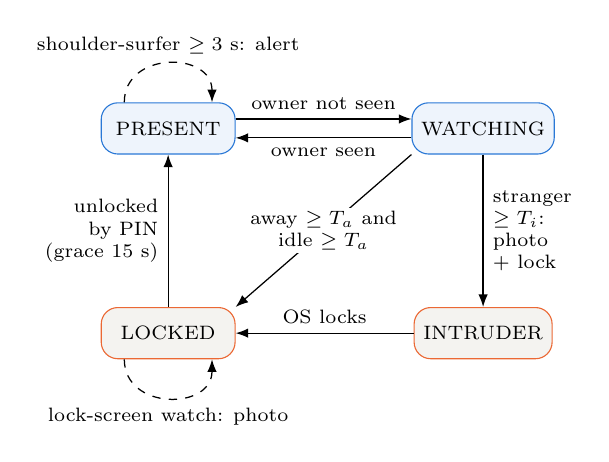
\begin{tikzpicture}[x=1mm, y=1mm,
  font=\scriptsize,
  st/.style={draw=fgblue, fill=fgfill, rounded corners=6pt, minimum width=17mm, minimum height=6.5mm, align=center},
  al/.style={draw=fgorange, fill=fggrey, rounded corners=6pt, minimum width=17mm, minimum height=6.5mm, align=center},
  lab/.style={fill=white, inner sep=1pt, align=center},
  arr/.style={-{Latex[length=1.6mm]}, line width=0.45pt}]
\node[st] (present) at (0,0)    {PRESENT};
\node[st] (watch)   at (40,0)   {WATCHING};
\node[al] (lock)    at (0,-26)  {LOCKED};
\node[al] (intr)    at (40,-26) {INTRUDER};
\draw[arr] ([yshift=1.2mm]present.east) -- node[above]{owner not seen} ([yshift=1.2mm]watch.west);
\draw[arr] ([yshift=-1.2mm]watch.west) -- node[below]{owner seen} ([yshift=-1.2mm]present.east);
\draw[arr] (watch) -- node[right, align=left]{stranger\\ $\ge T_i$:\\ photo\\ + lock} (intr);
\draw[arr] (watch.south west) -- node[lab, pos=0.5]{away $\ge T_a$ and\\ idle $\ge T_a$} (lock.north east);
\draw[arr] (intr) -- node[above]{OS locks} (lock);
\draw[arr] (lock) -- node[left, align=right]{unlocked\\ by PIN\\ (grace 15 s)} (present);
\draw[arr, dashed] ([xshift=3mm]present.north west) to[out=90, in=90, looseness=1.5] node[above]{shoulder-surfer $\ge3$ s: alert} ([xshift=-3mm]present.north east);
\draw[arr, dashed] ([xshift=3mm]lock.south west) to[out=-90, in=-90, looseness=1.5] node[below]{lock-screen watch: photo} ([xshift=-3mm]lock.south east);
\end{tikzpicture}
\caption{Presence-guard states (simplified; PAUSED, NO\_CAMERA and NO\_OWNER omitted). Solid arrows change state, dashed arrows raise alerts.}
\label{fig:guard}
\end{figure}

\begin{algorithm}[!t]
\caption{Presence-guard update (4 frames per second)}\label{alg:guard}
\footnotesize
\begin{algorithmic}[1]
\Require labeled tracked faces, idle time $I(t)$, session state
\Ensure possibly a lock, a photograph or a notification
\If{the session is locked}
  \IfThen{within $W$ min of locking and a stranger is confirmed}{photograph it}
  \State \Return
\EndIf
\IfThen{an authorized face is visible}{$t_a\gets t$}
\If{$\min(t-t_a, I(t))\ge T_a$} lock the PC (warning at $T_a-8$~s)
\ElsIf{a quality-checked stranger is seen for $T_i$, $t-t_a\ge3$~s, outside the grace period, $<3$ locks in 10 min}
  \State photograph, notify and lock the PC
\ElsIf{an authorized face and a stranger $\ge40$~px are seen for 3~s}
  \State notify (at most once per minute)
\EndIf
\end{algorithmic}
\end{algorithm}

\emph{Implementation.} OpenCV runs the YuNet (\texttt{face\_detection\_yunet\_2023mar}, 0.23~MB) and SFace (\texttt{face\_recognition\_sface\_2021dec}, 38.7~MB) models in the Open Neural Network Exchange (ONNX) format, and the MediaPipe Face Landmarker (\texttt{face\_landmarker.task}, 3.8~MB) supplies 478 points and 52 blendshape scores. Template files are written atomically with a backup copy. The application offers a live view with landmark, mesh and head-pose overlays, guided enrollment, face unlock, people management, the presence guard, an intruder gallery and a ``Model Lab'' that shows leave-one-out accuracy, score histograms and an embedding map of the user's own gallery (Fig.~\ref{fig:screens}). All functions are also available from the command line. The code base has about ten thousand lines of Python and 110 automated tests.

\begin{figure}[!t]
\centering
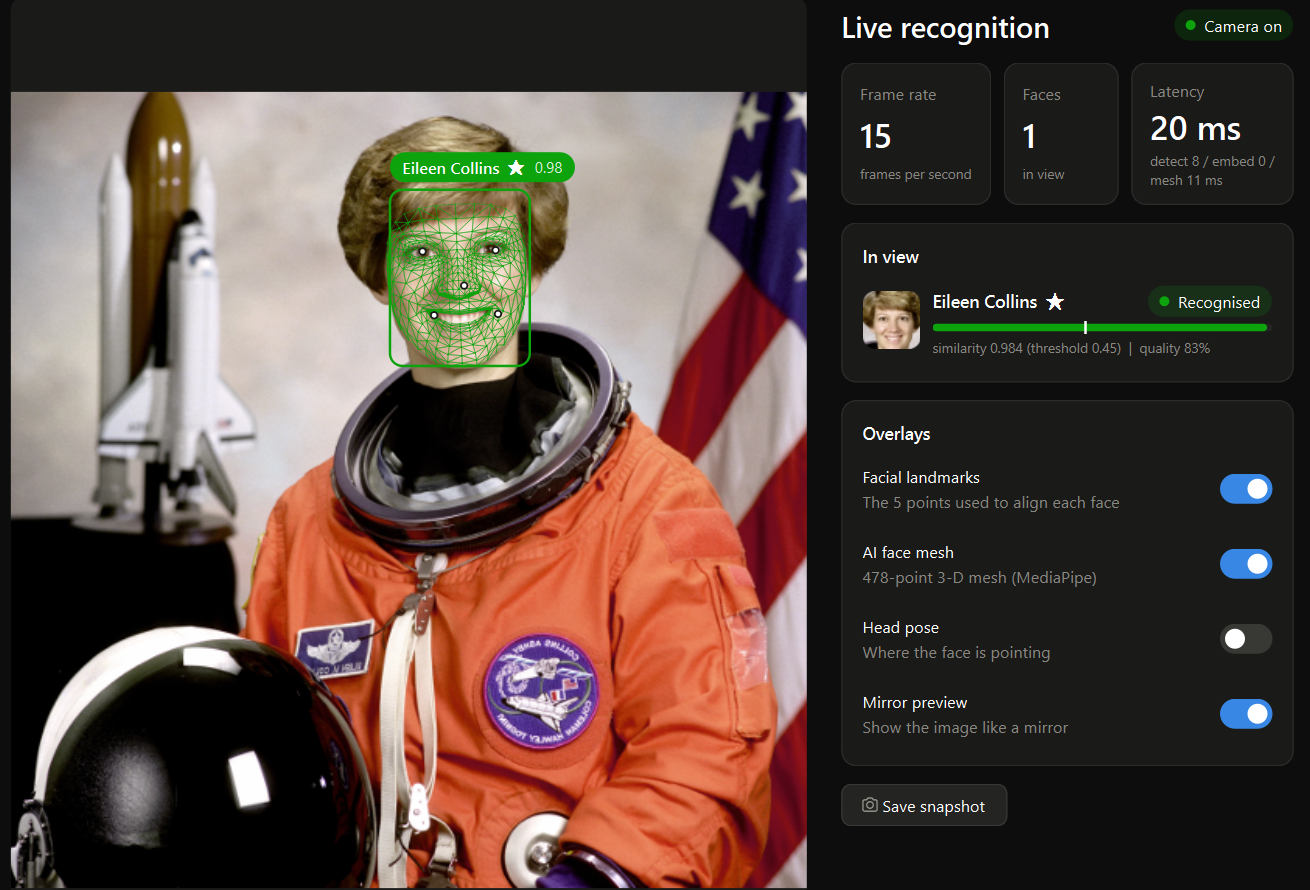
\includegraphics[width=\columnwidth]{figures/screen_live_crop.png}\\[3pt]
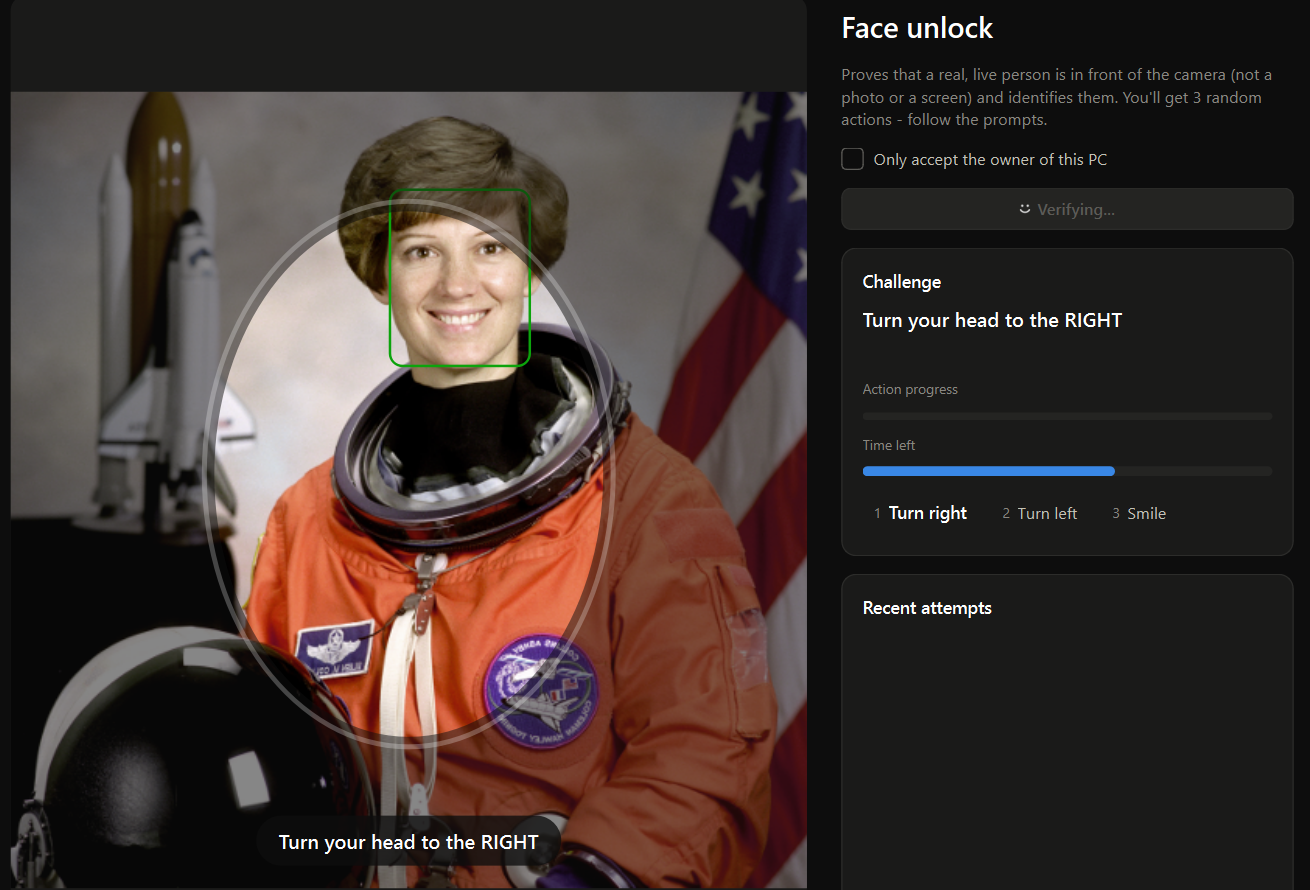
\includegraphics[width=\columnwidth]{figures/screen_unlock_crop.png}
\caption{\sys{} user interface (navigation bar cropped). Top: live recognition with the 478-point face mesh, the identity label with its similarity meter and threshold marker, and the per-stage latency. Bottom: a face-unlock session prompting a head turn, for which a still photograph cannot produce the required parallax. The camera input is replaced here by a public-domain NASA portrait.}
\label{fig:screens}
\end{figure}

% =====================================================================================================
\section{Recognition}\label{sec:s-recog}

\emph{Data details.} The \lfwImages{} LFW photographs show \lfwPeople{} individuals. YuNet found a face in every image; in the \lfwMultiFace{} images with several faces, the one nearest to the image center was used. In the median, faces are \lfwFaceWidth{} pixels wide and turned by \lfwYawMedian$^\circ$. The head-pose agreement reported in Section~III-C was measured on the \poseN{} of 3,000 randomly sampled LFW images for which MediaPipe returned a mesh.

\emph{Identification and robustness protocols.} Identification involves the \idPeople{} people with ten or more images (\idImages{} images in total) and $g$ enrollment images each, averaged over five repetitions. For the open-set test, half of these people (\osEnrolled{}) are enrolled with five images, and the probes are their remaining images (\osKnown{} on average) together with every image of the others (\osUnknown{}). Robustness is measured on the \robPairs{} pairs of View-2 splits 1 and 2 with only the probe degraded; in addition, every degraded probe is compared with \robImpGallery{} clean images of other people, giving \robImpN{} impostor comparisons per condition.

\emph{Verification.} Fig.~\ref{fig:roc} shows the ROC curves of the SFace variants of Table~I, Table~\ref{tab:op} the operating points of the three security levels on single LFW image pairs, and Fig.~\ref{fig:scores} the underlying score distributions.

\begin{figure}[!t]
\centering
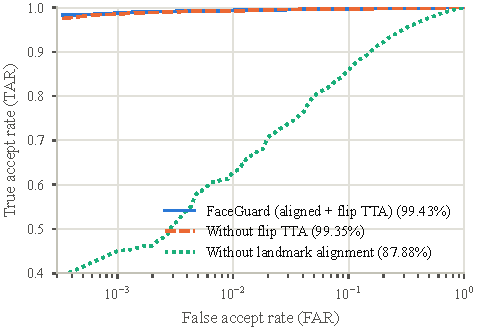
\includegraphics[width=\columnwidth]{figures/fig_roc.pdf}
\caption{ROC curves of the SFace pipeline on LFW View~2 (accuracy in brackets). Landmark alignment is essential; flip test-time augmentation (TTA) adds a small gain.}
\label{fig:roc}
\end{figure}

\begin{table}[!t]
\centering
\caption{Operating Points on LFW Image Pairs (\opGenuine{} Genuine and \opImpostor{} Impostor Pairs)}
\label{tab:op}
\footnotesize
\begin{tabular}{@{}lccc@{}}
\toprule
Security level & $\tau$ & FAR (\%) & FRR (\%) \\
\midrule
Relaxed & 0.38 & \farRelaxed & \frrRelaxed \\
Balanced (default) & 0.45 & \farBalanced & \frrBalanced \\
Strict & 0.52 & \farStrict & \frrStrict \\
\midrule
Windows Hello requirement~\cite{ms2024hello} & -- & $<0.001$ & $<5$ \\
\bottomrule
\end{tabular}
\end{table}

\begin{figure}[!t]
\centering
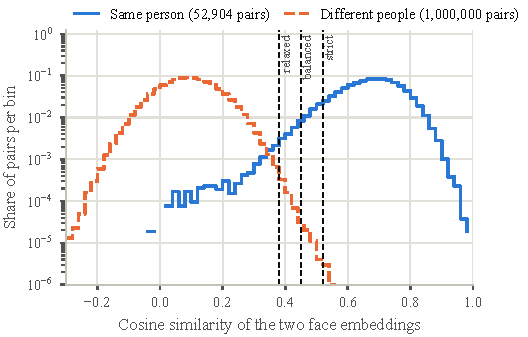
\includegraphics[width=\columnwidth]{figures/fig_scores.pdf}
\caption{Similarity distributions of \opGenuine{} genuine and \opImpostor{} impostor LFW pairs (log scale) with the three security thresholds.}
\label{fig:scores}
\end{figure}

\emph{Identification.} Closed-set identification is already \idOneNn\% correct with a single enrollment image and levels off near 99.9\% with two or more. Classifiers trained on the embeddings bring no meaningful gain: with five enrollment images a linear support vector machine reaches \clsSvm\%, logistic regression \clsLogreg\% and $k$-nearest neighbors \clsKnn\%, against \clsTopthree\% for the top-3 rule, and unlike the similarity rules they must be retrained for every new person and cannot reject strangers by design. The open-set test separates the rules more clearly (Fig.~\ref{fig:openset}, Table~\ref{tab:openset}). At the balanced threshold, the top-3 rule falsely accepts \osTopthreeFarBalanced\% of unseen people, about half the rate of the nearest-neighbor rule (\osNnFarBalanced\%), while identifying \osTopthreeDirBalanced\% of enrolled probes; at the strict level its false-alarm rate is \osTopthreeFarStrict\%. The centroid rule attains the highest detection-and-identification rate (DIR) at low false-alarm rates but depends on a representative enrollment, whereas the top-3 mean copes better with atypical samples and is therefore the default. False alarms are more frequent here than in Table~\ref{tab:op} because each probe is compared with every enrolled person, which is why the guard requires unknown faces to persist and face unlock requires a live, smoothed match.

\begin{figure}[!t]
\centering
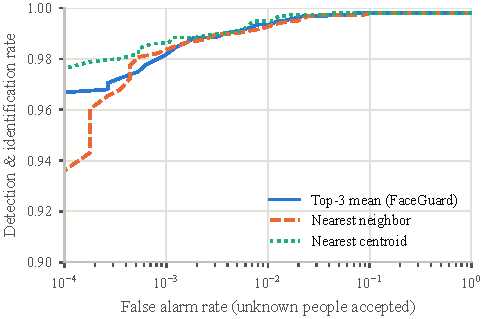
\includegraphics[width=\columnwidth]{figures/fig_openset.pdf}
\caption{Open-set identification on LFW: \osEnrolled{} enrolled people with five images each, probed by their other images and by \osUnknown{} images of unseen people.}
\label{fig:openset}
\end{figure}

\begin{table}[!t]
\centering
\caption{Open-Set Identification on LFW: DIR (\%) at Fixed False-Alarm Rate and DIR / False-Alarm Rate (\%) at the Security Levels}
\label{tab:openset}
\footnotesize
\setlength{\tabcolsep}{1.6pt}
\begin{tabular}{@{}lccccc@{}}
\toprule
Rule & DIR at & DIR at & Relaxed & Balanced & Strict \\
 & FAR 1\% & FAR 0.1\% & & & \\
\midrule
Nearest neighb. & \osNnDirTwo & \osNnDirThree & \osNnDirRelaxed/\osNnFarRelaxed & \osNnDirBalanced/\osNnFarBalanced & \osNnDirStrict/\osNnFarStrict \\
Top-3 (\sys) & \osTopthreeDirTwo & \osTopthreeDirThree & \osTopthreeDirRelaxed/\osTopthreeFarRelaxed & \osTopthreeDirBalanced/\osTopthreeFarBalanced & \osTopthreeDirStrict/\osTopthreeFarStrict \\
Centroid & \osCentroidDirTwo & \osCentroidDirThree & \osCentroidDirRelaxed/\osCentroidFarRelaxed & \osCentroidDirBalanced/\osCentroidFarBalanced & \osCentroidDirStrict/\osCentroidFarStrict \\
\bottomrule
\end{tabular}
\end{table}

\emph{Robustness to degradations.}\label{sec:s-robust} Fig.~\ref{fig:robust} shows verification with degraded probes at the balanced threshold, where clean probes give \robClean\% TAR. Darkness hardly matters (\robGainLow\% TAR at 15\% brightness), whereas over-exposure does (\robGainThree\% at three times the brightness), which motivates the asymmetric exposure limits of the quality gate. Recognition holds for faces down to about \robScaleQuarterPx{} pixels in width (\robScaleQuarter\% TAR), while detection breaks down below roughly \robScaleSmallPx{} pixels, where only \robScaleSmallDet\% of faces are found. Gaussian blur of 4 pixels, JPEG quality 4 and noise with a standard deviation of 32 gray levels reduce the TAR to \robBlurFour\%, \robJpegFour\% and \robNoiseThirtyTwo\%, respectively. A mask-like occluder over the lower face keeps \robMask\% TAR and sunglasses \robSunglasses\%, with AUCs of \robMaskAuc{} and \robSunglassesAuc{}, so occlusion harms a fixed threshold more than it harms the ranking of scores.

On the \robImpN{} impostor comparisons per condition, clean probes produced \robFaClean{} false accepts (FAR \robFarLargeClean\%). Severe degradations lowered the FAR (at most \robFarSevereMax\% for blur of 4 or 6 pixels, three-fold over-exposure, down-scaling to 12\%, JPEG quality 4 or noise of 32 gray levels), whereas mild ones left it of the same order; the highest value, \robFarLargeMax\% (\robFarWorstFa{} false accepts) for down-scaling by a factor of \robFarWorstLevel, remains below the pairwise FAR of the balanced level in Table~\ref{tab:op}. Degraded probes are therefore mostly rejected rather than confused with other people, but mild down-scaling does not by itself make the system safer.

\begin{figure*}[!t]
\centering
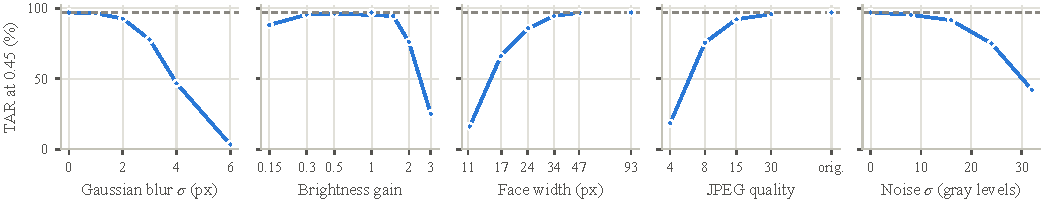
\includegraphics[width=\textwidth]{figures/fig_robust.pdf}
\caption{Robustness of verification at the balanced threshold ($\tau=0.45$) when the probe is degraded (\robPairs{} LFW pairs, enrollment image clean). The dashed line is the clean-probe TAR.}
\label{fig:robust}
\end{figure*}

% =====================================================================================================
\section{Liveness}\label{sec:s-liveness}

\emph{Simulation details.} The simulated head faced the camera, turned at a random speed and, when the progress bar stalled, turned further or blinked harder. Each print configuration was attacked \attPrintN{} times and the two replay attacks were run \attReplayN{} and \attUniversalN{} times; live users were simulated in \livN{} sessions for the default protocol and in \livNAbl{} sessions per ablation.

\emph{Sensitivity to the behavioral model.} Table~\ref{tab:sens} varies the behavioral model of simulated live users. The BPCER is unchanged for median reaction delays of 0.5 and 1.0~s (\sensReactFast\% and \sensReactSlow\%) and stays low for larger turns (\sensAmpLarge\% at $38^\circ$) or occasional confusion (\sensConfTen\% at 10\%); it rises to \sensReactSlowest\% for very slow users (1.4~s), \sensAmpSmall\% for timid turns of $22^\circ$ and \sensConfTwenty\% when left and right are confused in 20\% of prompts. Landmark noise and stricter turn thresholds also raise rejections (Fig.~\ref{fig:liveness}(a)); with 2-pixel noise the BPCER of the default protocol is \livFrrNoise\%. A session lasted \livTime~s on average (Fig.~\ref{fig:liveness}(b)).

\begin{table}[!t]
\centering
\caption{Sensitivity of the BPCER (\%) to the Behavioral Model of Live Users (Default Values in Bold)}
\label{tab:sens}
\footnotesize
\setlength{\tabcolsep}{4pt}
\begin{tabular}{@{}lcccc@{}}
\toprule
Median reaction delay (s) & 0.5 & \textbf{0.7} & 1.0 & 1.4 \\
BPCER & \sensReactFast & \textbf{\livFrr} & \sensReactSlow & \sensReactSlowest \\
\midrule
Mean turn amplitude ($^\circ$) & 22 & \textbf{30} & 38 & \\
BPCER & \sensAmpSmall & \textbf{\livFrr} & \sensAmpLarge & \\
\midrule
Left/right confusion (\%) & 0 & \textbf{5} & 10 & 20 \\
BPCER & \livFrrNoConf & \textbf{\livFrr} & \sensConfTen & \sensConfTwenty \\
\bottomrule
\end{tabular}\\[2pt]
\raggedright\scriptsize 1,000 simulated users per non-default setting (\livN{} for the default).
\end{table}

\begin{figure*}[!t]
\centering
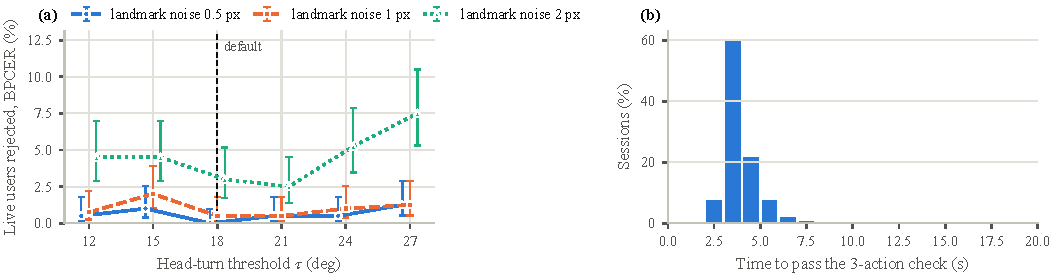
\includegraphics[width=\textwidth]{figures/fig_liveness.pdf}
\caption{Live-user rejection. (a) BPCER against the head-turn threshold for three levels of landmark noise (turn-only protocol, 400 sessions per point, 95\% Wilson intervals). (b) Time needed to pass the default three-action check (\livN{} sessions).}
\label{fig:liveness}
\end{figure*}

\emph{Pose jitter.} Under sensor noise of 4 gray levels, the yaw estimate of a still face fluctuates by \poseJitter$^\circ$ on average (95th percentile \poseJitterQ$^\circ$), far below the $18^\circ$ turn threshold.

% =====================================================================================================
\section{Presence Guard and Runtime}\label{sec:s-guard}

\emph{Guard simulation.} Table~\ref{tab:guard} gives the full results of the guard simulation of Section~V-G. In the owner-at-the-desk scenario the owner was labeled unknown in \gUnknownFrac\% of frames, but an authorized face was present in every frame (longest period without one: \gLongestGap~s, against $T_a=30$~s), so the frames labeled unknown are frames in which the largest face in view was another person in the photograph. Re-running the production engine on the streamed photographs traced the \gShldAlerts{} shoulder-surfer alerts to the \gdSecond{} of \gdPhotos{} images (\gdSecondPct\%) in which a second, unknown person at least 40~pixels wide is visible; cues such as gaze direction or distance could make the rule more selective.

Classifying each trial's stranger with the production engine explains every miss of the intruder and onlooker trials: the quality gate rejected the photograph in \gdIntrQuality{} and \gdShldQuality{} trials and the score fell in the uncertain band in \gdIntrUncertain{} and \gdShldUncertain{} trials, respectively, while no stranger was ever accepted as the owner. The replacement trials, which reuse the same strangers, missed \gReplExtra{} more.

\begin{table}[!t]
\centering
\caption{Presence Guard on Simulated Webcam Streams (Production Engine and Thresholds, 4 Frames per Second)}
\label{tab:guard}
\footnotesize
\setlength{\tabcolsep}{3pt}
\begin{tabular}{@{}lr@{}}
\toprule
\multicolumn{2}{@{}l}{Owner at the desk: \gOwners{} owners, \gHours{}~h, \gFrames{} frames} \\
\quad frames: owner / uncertain / unknown (\%) & \gMatchFrac{} / \gUncertainFrac{} / \gUnknownFrac{} \\
\quad false intruder locks per hour & \gFalseIntruder \\
\quad false walk-away locks per hour, no typing & \gFalseWalk \\
\quad longest time without recognition (s) & \gLongestGap \\
\quad shoulder-surfer alerts per hour (see text) & \gShldAlertsHour \\
\midrule
\multicolumn{2}{@{}l}{Stranger sits down 5~s after the owner left (\gIntrN{} trials)} \\
\quad locked within 20~s (\%) & \gIntrRate \\
\quad time to lock: median / mean / 95th pct.\ (s) & \gIntrMed{} / \gIntrMean{} / \gIntrQ \\
\multicolumn{2}{@{}l}{Stranger replaces the owner without a gap (\gReplN{} trials)} \\
\quad locked within 20~s (\%) & \gReplRate \\
\quad time to lock: median / mean / 95th pct.\ (s) & \gReplMed{} / \gReplMean{} / \gReplQ \\
\multicolumn{2}{@{}l}{Shoulder-surfer behind the owner (\gShldN{} trials)} \\
\quad alerted within 20~s (\%) & \gShldRate \\
\quad time to alert: median / 95th pct.\ (s) & \gShldMed{} / \gShldQ \\
\bottomrule
\end{tabular}\\[2pt]
\raggedright\scriptsize Latencies are quantized to the 0.25~s frame interval, so the median and the 95th percentile can coincide.
\end{table}

\emph{Runtime.} Fig.~\ref{fig:runtime} breaks down the latency at the default $640\times480$ resolution: detection takes \rtDet~ms, alignment \rtAlign~ms and one embedding \rtEmb~ms, or \rtEmbTta~ms with mirroring. A frame of the complete pipeline costs \rtPipe~ms on average, \rtPipeAll~ms if every frame is re-embedded and \rtPipeMesh~ms with the face mesh. The live view ran at \rtFps{} frames per second with a total CPU load of \rtCpuLive\%, while the background guard at four frames per second used \rtCpuGuard\% (\rtCpuGuardCore\% of one core). Loading the recognition models takes \rtLoad~ms and the mesh model \rtLoadMesh~ms. With flip TTA and default threading, an SFace embedding of an aligned crop takes \baseSfaceMs~ms, an ArcFace MobileFaceNet embedding \baseMbfMs~ms and an ArcFace ResNet-50 embedding \baseRfiftyMs~ms. Runtimes are means of 200 runs after 20 warm-up runs on an otherwise idle machine; the CPU load of the live view was measured with a synthetic 30-frame-per-second image stream instead of a physical camera.

\begin{figure}[!t]
\centering
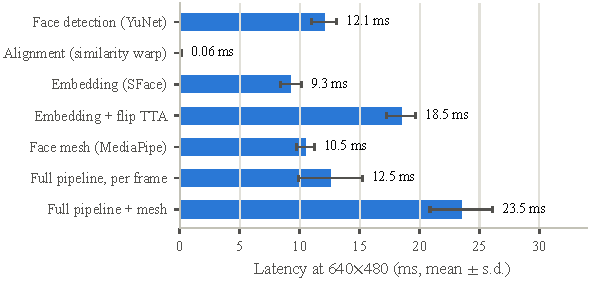
\includegraphics[width=\columnwidth]{figures/fig_runtime.pdf}
\caption{Latency of each stage on the laptop CPU at $640\times480$ (200 runs). The full pipeline re-embeds each tracked face every 0.35~s.}
\label{fig:runtime}
\end{figure}

% =====================================================================================================
\section{Reproducibility}\label{sec:s-repro}

\emph{Software.} The software is written in Python~3.12 with OpenCV~5.0, NumPy~2.5, MediaPipe~1.0.1, scikit-learn~1.9.1 and PySide6~6.11; the ArcFace baselines use onnxruntime~1.30. Every model is checked against a pinned SHA-256 hash after download.

\emph{Seeds.} Every randomized step uses a fixed seed: 2026 for the impostor pairs, the identification repetitions, the calibration/evaluation split of the face meshes, the MPIIFaceGaze sample and the demographic impostor pairs; 0 for the mesh selection; 17 for the robustness impostor gallery; 70 and 7 for the two guard scenarios; and one recorded seed per Monte-Carlo configuration.

\emph{Code and data.} The experiment scripts regenerate every number, table and figure of the main article from the public datasets, which are downloaded separately under their own licenses (LFW, MPIIFaceGaze, LFW attribute labels) together with the pretrained models. The raw logs of the real-world pilot are not released because they contain per-frame facial landmarks of a participant; their anonymous summary, from which Table~VII of the main article is computed, is included.

\bibliographystyle{IEEEtran}
\bibliography{references}

\end{document}
